\documentclass{exam} 
\printanswers 
\def\workshopTitle{Workshop - Introduction} 
\input{comp125workshopHeader} 
\section*{Learning outcomes}
Most of you have done COMP115 at Macquarie with Processing as the programming language and environment. We will revise some of the basics of programming learnt in COMP115. Also, in COMP125, Java is the programming language and Eclipse is the environment. Following are this week's learning outcomes,
\begin{enumerate}
\item 15 minutes: introductions
\item 10 minutes: be ready to use the lab computers (setup accounts and iLearn)
\item 50 minutes: revise COMP115/WCOM115 topics
\item 20 minutes: create a simple java program in Eclipse and under
\item 15 minutes: import a java project in Eclipse
\end{enumerate}

\vspace{1em}
\begin{questions}
\question  \textbf{Access your account} \vskip 0.5cm
To log on to the lab machines, first make sure the machine is powered on. 
Enter your username (OneID) and password in the appropriate entry boxes. 
Please note that if you have already accessed the labs, your username and password are the same as in the previous semester, and if are accessing the labs for the first time, you should have the required information from enrolment/ orientation session. If you do not have this information, please ask the tutor to assist you.

Once you login to the computer, make sure you have access to COMP125 homepage in iLearn. If not, please ask the tutor to assist you.

\newpage

\section*{COMP115/ WCOM115 Revision}

\question What is the value of \texttt{result} when the following code is executed?
\begin{lstlisting}
int result = 12/5;
\end{lstlisting}

\begin{solution}
2 (integer/integer = integer)
\end{solution}

\question What is the value of \texttt{result} when the following code is executed?
\begin{lstlisting}
float result = 12/5;
\end{lstlisting}

\begin{solution}
2.0 (integer/integer = integer, and then that integer (2) is copied into a \texttt{float})
\end{solution}

\question What is the value of \texttt{result} when the following code is executed?
\begin{lstlisting}
float result = 12.0/5;
\end{lstlisting}

\begin{solution}
2.4 (float/integer = float (2.4), and then that float (2.4) is copied into a \texttt{float})
\end{solution}

\question Consider the following code:
\begin{lstlisting}
size(300, 200);
background(255);
int x = (int)random(width);
int y = (int)random(height);
if(x < width/2) {
	if(y < height/2) {
		line(0, 0, x, y);
	}
	else {
		ellipse(x, y, 20, 20);
	}
}
else {
	if(y < height/2) {
		rect(x, y, 20, 20);
	}
	else {
		triangle(x, 0, x, y, 0, y);
	}
}
\end{lstlisting}

Give 4 samples of \texttt{(x, y)} pairs, such that for each pair a different shape is drawn. Also state which shape is drawn for which \texttt{(x, y)} pair.
\begin{solution}
\begin{itemize}
	\item (20, 20): line
	\item (20, 120): ellipse (circle)
	\item (180, 20): rectangle
	\item (180, 120): triangle
\end{itemize}
\end{solution}

\question What is the value of \texttt{result} when the following code is executed?
\begin{lstlisting}
int result = 1;
for(int i=0; i<4; i++) {
	result*=2;
}
\end{lstlisting}

\begin{solution}
16 (loop executes four times, for \texttt{i = 0, 1, 2, 3} and each time \texttt{result} doubles).
\end{solution}

\question What is the value of \texttt{result} when the following code is executed? Can you state the value of \texttt{result} in terms of \texttt{n}?
\begin{lstlisting}
int n = 64;
int result = 0;
for(int i=1; i*i<=n; i++) {
	result++;
}
\end{lstlisting}

\begin{solution}
\texttt{result = 8}. More generally, \texttt{result = }$\sqrt{{n}}$. This is when \texttt{n} is a perfect square. If \texttt{n} is not a perfect square, then \texttt{result = }$\sqrt{{\lfloor n \rfloor}}$
\end{solution}

\question What is the value of \texttt{result} when the following code is executed? Draw a memory diagram to illustrate the memory transactions that occur during the function call. Refer to the document \texttt{functions.pdf} released in the revision package to help you with the diagram.
\begin{lstlisting}
int foo(int a, int b) {
	if(a < b)
		return a;
	else
		return b;
}
\end{lstlisting}

\begin{lstlisting}
int p = 6;
int q = 3;
int result = foo(p - 2, q + 2);
\end{lstlisting}

\begin{solution}
Function call: foo(4, 5)
a is 4
b is 5
expression inside if condition is true
returned value: a (4), copied into result, which becomes 4
\end{solution}

\question Write a function that when passed an integer, \texttt{true} if it is even (divisible by 2), and \texttt{false} otherwise.
\begin{solution}
\begin{lstlisting}
boolean isEven(int n) {
	if(n % 2 == 0) {
		return true;
	}
	else {
		return false;
	}
}
\end{lstlisting}	
\end{solution}

\newpage

\question Write a function that when passed an integer and a boolean, returns:

\begin{itemize}
	\item if the boolean value is \texttt{true}, then the square of the integer
	\item otherwise
			\begin{itemize}
				\item if the integer is positive, then the integer itself
				\item otherwise, negative of the integer
			\end{itemize}
\end{itemize}

\begin{solution}
\begin{lstlisting}
int moo(int a, boolean b) {
	if(b) {
		return a*a;
	}
	else {
		if(a > 0) {
			return a;
		}
		else {
			return -a;
		}
	}
}
\end{lstlisting}
\end{solution}

\question Draw the memory diagram that illustrates the arrays stored in the memory for the following code:

\begin{lstlisting}
int[] a = {10, 70, 20, 90, 30};
int[] b = {a[2], a[1], a[0]};
int[] c = b;
\end{lstlisting}

\begin{solution}
\begin{tikzpicture}
\memoryblock{y=4, width=2, height=1,array={"a"}, colour = white!80!red}
\memoryblock{x=3, width=2, height=5,array={"[0] = 10", "[1] = 70", "[2] = 20", "[3] = 90", "[4] = 30"}}
\arrow{startX=1.8, startY=4.5, endX=3, endY=4.5}
\memoryblock{x=10, y=4, width=2, height=1,array={"b"}, colour = white!80!red}
\memoryblock{x=7, width=2, height=4,array={"[0] = 30", "[1] = 20", "[2] = 10"}}
\arrow{startX=10.2, startY=4.5, endX=9, endY=3.5}
\memoryblock{x=10, y=2, width=2, height=1,array={"c"}, colour = white!80!red}
\arrow{startX=10.2, startY=2.5, endX=9, endY=3.5}
\end{tikzpicture}
\vskip 0.5cm
\end{solution}

\question 

\begin{enumerate}
\item Declare an array \texttt{arr} to store integers. 
\item Instantiate it to hold 400 integers. 
\item Using a loop, initialize the items such that the first item is 10, second item is 15, third item is 20 and so on ...
\end{enumerate}

\begin{solution}
\begin{lstlisting}
int[] arr; //declaration

arr = new int[400]; //instantiation

int val = 10; //value for first item

for(int i=0; i < arr.length; i++) { //populating the array
	arr[i] = val;
	val = val + 5;
}

/*
you can also do it without need for variable val as:
for(int i=0; i < arr.length; i++) { //populating the array
	arr[i] = 10 + i*5;
}
*/
\end{lstlisting}
\end{solution}

\question What is the state of the array \texttt{a} when the following code is executed?

\begin{lstlisting}
float[] a = {2.5, 2.2, -3.4, 0, 6.8};
for(int i=1; i < a.length; i++) {
	if(a[i] > 0) {
		a[i] = a[i] - 3;
	}	
	if(a[i] < 0) {
		a[i] = a[i] - 1;
	}
	else {
		a[i] = a[i] + 1;
	}
}
\end{lstlisting}

\begin{solution}
\texttt{\{2.5, 0.2, -2.4, 1, 2.8\}}

Note that first item is not changed since the loop started from \texttt{i = 1}.	
\end{solution}

\newpage

\question Writing, compiling and executing a simple Java program 

The structure of a basic java program is as follows:

\begin{lstlisting}[numbers=none]
//filename: HelloWorld.java
public class HelloWorld {
	public static void main(String[] args) {
		//FIXME
	}
}
\end{lstlisting}

The meaning of each of the components will be covered in the lecture. Write now, you can focus on replacing the comment FIXME with your code. 

\begin{enumerate}
	\item Copy the code above
	\item Open text editor "Atom" installed in lab computers
	\item Paste the copied code
	\item Fix the indentation
	\item Save it as "HelloWorld.java" under a convenient directory (Say "Documents"). If the class name is \texttt{HelloWorld}, it \textbf{must} be in a file named \texttt{HelloWorld.java} (and \textbf{not} \texttt{helloWorld.java} or \texttt{helloworld.java} or \texttt{Helloworld.java}).
	\item Replace the comment FIXME with the statement,
		\begin{lstlisting}
System.out.println("Hello World");
		\end{lstlisting}
	\item Save
	\item Exit.
\end{enumerate}

Next, to \emph{compile} and \emph{execute} the program. 

The following diagram describes the process of compiling a java source code (.java) into java bytecode (.class) and then executing the bytecode on the Java Virtual Machine (JVM).
\vskip 0.5cm
\begin{center}
	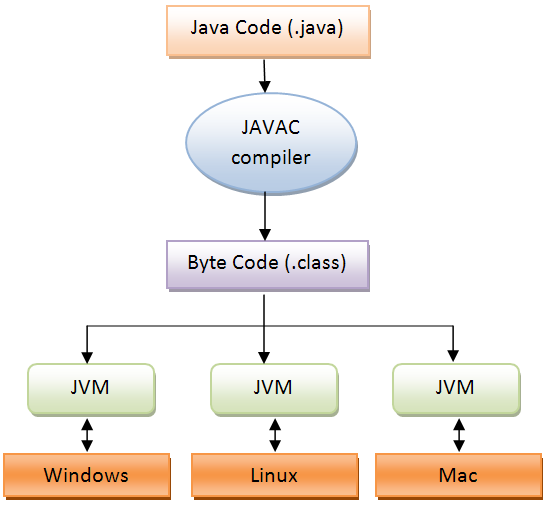
\includegraphics[scale=0.3]{javaCompileExecute}
\end{center}
\vskip 0.5cm

Open Command Prompt/ PowerShell and go to the folder in which you saved the java file. Run the following command (or \texttt{ls} on a Mac/Linux) to list the contents of the directory:

\begin{lstlisting}[numbers=none]
dir
\end{lstlisting}

You should see the file (amongst others)

\begin{lstlisting}[numbers=none]
HelloWorld.java
\end{lstlisting}

Type the following command to compile \texttt{HelloWorld.java}. 

\begin{lstlisting}[numbers=none]
javac HelloWorld.java	
\end{lstlisting}

If everything is ok, you won't see any error message and if you run the \texttt{dir} command again, you will see the additional file

\begin{lstlisting}[numbers=none]
HelloWorld.class
\end{lstlisting}

If you *do* see an error message, take a look at the error message and fix the corresponding line. Ask your peers or tutor to help you if required.

Once the errors (if any) are fixed, type the following command to run/execute \texttt{HelloWorld.class}. 

\begin{lstlisting}[numbers=none]
java HelloWorld
\end{lstlisting}

IMPORTANT: NO ".class" in the execution command.

Now, repeat the process with \texttt{Program1.java}. After compiling and running, you should see the following output:

\begin{lstlisting}[numbers=none]
number: 147
number of digits: 3
\end{lstlisting}

Now, repeat the process with \texttt{Program2.java}. You will see that the compilation doesn't succeed and that there are errors.

Open the file \texttt{Program2.java} in either Atom text editor (preferred) or WordPad (not Notepad).

Figure out the problems in the program, fix and compile until you succeed.

Once the compilation is finished, run the program. You will see the following output (which is incorrect):

\begin{lstlisting}[numbers=none]
n = 6
sum of integers from 1 to 6: 15	
\end{lstlisting}

Go back to the program, fix the logical error, and run the program again.

You will notice that the output is unchanged (WHAT!?!?!?!?)

Every time we update the source code (.java), we must recompile the program before executing it.

So, compile the updated program again, and execute it. Now you should get the correct output:

\begin{lstlisting}[numbers=none]
n = 6
sum of integers from 1 to 6: 21
\end{lstlisting}

Repeat the process with \texttt{Program3.java}.

\question \textbf{Writing your first java program in Eclipse (pair-programming)} \vskip 0.5cm

\begin{enumerate}
\item Follow the instructions in video uploaded \href{https://www.youtube.com/watch?v=8DcIQcmwuSE}{here} to create your first program in Eclipse that displays the following message in the console:

\begin{verbatim}
Bow before <person 1 name> and <person 2 name>
\end{verbatim}

So if your names are Bender Rodriguez and Philip J. Fry (since this exercise is being done in pairs, and if you didn't find a partner, choose your favourite character's name), the message should be

\begin{verbatim}
Bow before Bender Rodriguez and Philip J. Fry
\end{verbatim}

\item Make sure there are no red-crosses on any line of your code (red crosses imply syntactical error and are demons hiding in your computer).

\item Compile and Run your program
\end{enumerate}

\newpage

\question \textbf{Importing Java project from archive file} \vskip 0.5cm

Follow the following instructions to import Java project contained in \texttt{workshop01demoProgram.zip} archive file.

\begin{enumerate}
	\itemsep0.3em 
\item Download \texttt{workshop01code.zip}. \textbf{\color{red} DO NOT UNZIP IT} \color{black}.
\item Open \texttt{Eclipse} IDE. A shortcut for it should be located on your desktop.
\item If prompted, set your \texttt{workspace} (a location where all your projects will be saved). We suggest you use a dedicated folder in your network drive as the workspace.
\item Click on \color{blue} File --> Import --> General --> Existing Projects into workspace \color{red} (and NOT ``Archive file") \color{black}.
\item On the next window, choose ``Select archive file'' option and browse for the archive file \texttt{workshop01code.zip} and choose \texttt{Open}.
\item It should show projects \texttt{workshop01exercise} and \texttt{arrayHelp}. Click on \texttt{Finish}.
\item You should see a project in Eclipse in the left panel (\texttt{Package Explorer}).
\item Double click on the \texttt{workshop01exercise} to reveal \texttt{src}. \texttt{"src"} is short for \texttt{"source"} (that is, source code).
\item Double click on the \texttt{src} to reveal package \texttt{"(default package)"}.
\item Double click on the \texttt{(default package)} to reveal source file \texttt{TaskToDo}.
\item Your job is to complete the following methods (description in java file) in this class (you only need to write code inside the methods). Note the method headers are written in form \texttt{methodName(<parameterTypes>): <returnType>}.

\begin{enumerate}
\item \texttt{sum(int[]): int}
\item \texttt{sumEven(int[]): int}
\item \texttt{count(int[], int): int}
\item \texttt{contains(int[], int): boolean}
\item (Challenging) \texttt{countUnique(int[]): int}
\end{enumerate}

We have supplied a sample array in the \texttt{main} method and called the above methods in it by passing this array. Expected values are provided as comments next to these invocations. This is just a \textbf{sample data} and we will test your program by passing other arrays to the methods.

A separate java project (\texttt{week1arrayHelp}) is provided with the workshop package and can be imported in the same way as the other archive files.

\begin{solution}
Refer to \texttt{workshop01solutionCode.zip}	
\end{solution}
\end{enumerate}
\end{questions}

\newpage

\section*{Advanced questions (D/HD)}

\begin{questions}

\question Add a piece of code in the \texttt{main} method of class \texttt{TaskToDo}  that performs the following tasks,

\begin{enumerate}
\item creates an array to hold age of 20 people. 

\item assigns each value in the array to a random value between 1 and 100 (including 1 and 100). For this, a random number generator \texttt{rand} has been created for you and you can generate a random value between 1 and 100 using \texttt{rand.nextInt(100) + 1}. Display all values separated by a space on the console using \texttt{System.out.print(ages[i]+" ")} assuming \texttt{ages} is the name of the array.

\item displays the average age

\item computes the number of people under 50 years of age. Display this on the console using \texttt{System.out.println(var+'' people under 50 years of age'')} assuming you are storing the result in variable \texttt{var}. 

\item displays if there are two consecutive people aged over 80 years of age.

\item \textbf{(Advanced)} displays all unique ages. That is values that occur exactly once in the array.
\end{enumerate}

\begin{verbatim}

Sample output 1:

72 9 43 65 45 34 33 27 13 81 45 31 45 88 38 31 66 38 1 21 
Average age: 41.3
15 people under 50 years of age
Two consecutive people over 80: false
Items occurring exactly once:
72 9 43 65 34 33 27 13 81 88 66 1 21 

----------------------------

Sample output 2:

75 49 59 50 49 50 4 70 90 82 93 10 92 23 28 33 32 68 66 31 
Average age: 52.7
9 people under 50 years of age
Two consecutive people over 80: true
Items occurring exactly once:
75 59 4 70 90 82 93 10 92 23 28 33 32 68 66 31 
\end{verbatim}

\question Write a method that when passed two integer arrays, returns \texttt{true} if they are identical (exact same items in the same order), \texttt{false} otherwise.

\begin{solution}
\begin{lstlisting}
public static boolean identical(int[] a, int[] b) {
	if(a.length != b.length) {
		return false;
	}
		
	for(int i=0; i < a; i++) {
		if(a[i] != b[i]) {
			return false;
		}
	}
	
	return true;
}	
\end{lstlisting}	
\end{solution}

\question Write a method that when passed an integer array, returns an array containing the positive values in the array passed.

\begin{solution}
\begin{lstlisting}
public static int[] getPositives(int[] arr) {
	int count = 0;
	for(int i=0; i < arr.length; i++) {
		if(arr[i] > 0) {
			count++;
		}
	}
	
	int[] result = new int[count];
	
	int targetIndex = 0;
	
	for(int i=0; i < arr.length; i++) {
		if(arr[i] > 0) {
			result[targetIndex] = arr[i];
			targetIndex++;
		}
	}
	
	return result;
}
\end{lstlisting}	
\end{solution}

\question Write a method that when passed an array, returns the sub-array starting at the first index beyond which the array is in ascending order. For example, if the array passed is \texttt{\{40, 10, 80, 20, 70, 70, 90\}}, the method should return the array  \texttt{\{20, 70, 70, 90\}}.

\begin{solution}
\begin{lstlisting}
public static int[] getAscendingSubset(int[] arr) {
	int idx = 0;
	for(int i=0; i < arr.length - 1; i++) {
		if(arr[i] > arr[i+1]) {
			idx = i+1;
		}
	}
	
	int[] result = new int[arr.length - idx];
	
	for(int i=idx; i < arr.length; i++) {
		result[i - idx] = arr[i];
	}
	
	return result;
}
\end{lstlisting}	
\end{solution}

\end{questions}
\end{document}
